\chapter{Filtering Sound}

A feature any digital synthesizer should include is the possibility to filter sound. In digital signal processing, filtering a signal means to "alter [its] frequency spectrum [...] by amplifying or attenuating selected frequencies". \citebs{102} \vspace{\baselineskip}

The discussion of digital filters is closely linked to the concept of a signal's phase. More concretely, it must be examined how the phase relationship between two \emph{input} signals influences the properties of the \emph{output} signal produced when the two input signals interfere either constructively or destructively. A simple examples of phase relationships from the analog realm is the situation where signals $A$ and $B$ are exactly identical and consequently have a phase difference $\Delta \phi$ of $0$. If these signals are summed, the resulting signal $C$ will have an amplitude twice as high or low as that of signal $A$ or $B$ in every single point of its signal --- the input signals interfere \emph{constructively}. Conversely, if signals $A$ and $B$ have a phase difference of 180\degree or $\pi$ radians, the two signals interefere \emph{destructively} and result in signal $C$ having a constant amplitude of exactly $0$, as the amplitude values of signals $A$ and $B$ cancel each other out in each point of the signal. \vspace{\baselineskip}

In digital systems, where signals are represented discretely, i.e.\ with periodically recorded samples, a phase difference can be modeled by a \emph{sample delay}. \citebs{103} For example, if a signal that is periodically represented by 10 samples is summed with a version of itself that is delayed by 5 samples, that version will effectively be phase-shifted by 180\degree and thus the summation of these two signals will result in silence. Had only one sample been delayed instead of five, the phase difference $\Delta \phi$ would have only been 36\degree or $\frac{2\pi}{10}$ radians --- one tenth of a period. The amount of phase difference $\Delta \phi$ depends on both the number of samples a signal is represented by, so the sample rate of the system, and the number of samples that are delayed. An equation to calculate the phase difference in radians, given these parameters, is shown in Equation \ref{eq:phasediff}, where $f$ is the frequency of the signal, $f_{s}$ the sample rate and $N$ the number of samples that are delayed. If $2\pi$ is replaced by 360, this Equation yields the same phase difference in degrees.

\begin{equation}
  \Delta\phi = \frac{N \cdot f}{f_{s}} \cdot 2\pi
  \label{eq:phasediff}
\end{equation}

From Equation \ref{eq:phasediff} it can be deduced that a sample delay causes different phase relationships for different frequencies of the original signal. To give an example: let one sample be delayed in a system with a sample rate $f_{s}$ equal to 20 kHz. In such a system, a signal with a frequency of 1 Hz is represented by 20000 samples. Consequently, summing such a signal with a version of itself delayed by one sample would make the resulting, filtered signal almost twice as loud, as $\Delta\phi$ is only about 0.018\degree. However, a signal with the maximum possible frequency of 10 Khz (the Nyquist limit) is represented by only 2 samples. Therefore, delaying one sample equals a phase shift of 180\degree, which results in silence when the signal is summed with the delayed version of itself. This introduces the concept of a filter's \emph{frequency response}, which describes how a filter influences a signal's frequency spectrum. For the filter just described, the frequency response would look approximately like Figure \ref{fig:freqresp}. \vspace{\baselineskip}

\begin{figure}[t!]
  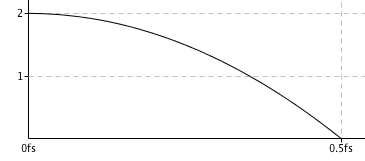
\includegraphics[scale=0.8]{img/freqresp}
  \caption{The frequency response of a one-sample-delay filter. The most constructive interference is at 0 Hz, a signal that is constant with $f(t) = 1$. Such a signal with a frequency of 0 Hz is also called DC, for direct current, because in analog circuits a DC current is constant. The most destructive interference occurs at $\frac{f_{s}}{2}$ Hz.}
  \label{fig:freqresp}
\end{figure}

One way to change the frequency response of a filter is to weight samples of the input signal as well as the delayed samples with \emph{filter coefficients} \citebs{105, 110}. Whereas previously a one-sample delay could be modeled by Equation \ref{eq:onedelay1} \citebs{104}, where $y_{n}$ is the output, $x_{n}$ the current and $x_{n-1}$ the delayed sample, Equation \ref{eq:onedelay2}, where $a$ and $b$ are the respective filter coefficients, must be used when samples are weighted with coefficients. \citebs{103} Visually, such a one-sample delay can be represented with the diagram shown in Figure \ref{fig:onedelay}.

\begin{equation}
  y_{n} = x_{n} + x_{n-1}
  \label{eq:onedelay1}
\end{equation}

\begin{equation}
  y_{n} = bx_{n} + ax_{n-1}
  \label{eq:onedelay2}
\end{equation}

\begin{figure}[h!]
  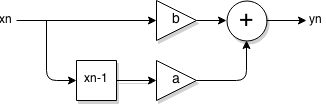
\includegraphics[scale=0.8]{img/onedelay}
  \caption{A one-sample delay with filter coefficients $a$ and $b$. Triangles are amplifiers/attenuators. Samples are summed at the circle with the + at its center.}
  \label{fig:onedelay}
\end{figure}

\pagebreak

\section{FIR and IIR Filters}

\noindent While a filter's frequency response describes how the frequency content of a signal is affected by that filter, its influence on a signal in the time domain is given by the filter's \emph{impulse response} or \emph{kernel}. More precisely, an impulse response determines what a filter outputs when its input is a delta function, $\delta$, which has a normalized \emph{impulse}, meaning a sample with an amplitude of 1, as its first sample while all other subsequent samples have an amplitude of 0. The $\delta$ function is also referred to as the \emph{unit impulse}. \citedsp{108} For example, if the filter coefficients of the three-sample delay filter shown in Figure \ref{fig:threedelay} are all equal to 0.5 ($a = b = c = 0.5$), leading to Equation \ref{eq:threedelay}, then Figure \ref{fig:impresp} gives the impulse response of this filter when it is fed the $\delta$ function depicted in Figure \ref{fig:deltafunc}. What this impulse response shows is that if a sample $x_{n}$ with an amplitude of 1 is input into this filter, the first sample output will be $1 + \frac{0}{2}+ \frac{0}{2}+ \frac{0}{2} = 1$. The second sample to exit this filter will then be $0 + \frac{1}{2}+ \frac{0}{2}+ \frac{0}{2} = 0.5$, where, following the definition of the $\delta$ function given above, the new $x_{n}$ is equal to 0, while the previous $x_{n}$ that was equal to 1 has moved into the position of $x_{n-1}$. The third sample will be equal to $0 + \frac{0}{2} + \frac{0.5}{2}+ \frac{0}{2} = 0.25$ and finally the fourth sample has a value of $\frac{1}{8}$.

\begin{equation}
  y_{n} = x_{n} + \frac{x_{n-1}}{2}+ \frac{x_{n-2}}{2}+ \frac{x_{n-3}}{2}
  \label{eq:threedelay}
\end{equation}

\begin{figure}
  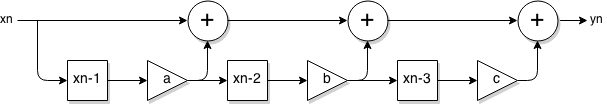
\includegraphics[scale=0.7]{img/threedelay}
  \caption{A three-sample delay filter.}
  \label{fig:threedelay}
\end{figure}

\begin{figure}

  \TopFloatBoxes

  \begin{floatrow}

    \ffigbox{\caption{A delta function, also called a unit impulse. The first sample has an amplitude of 1 while all other samples are equal to 0.} \label{fig:deltafunc}}{ 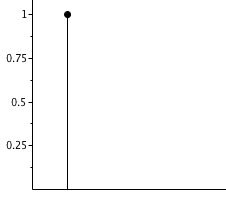
\includegraphics[scale=0.7]{img/deltafunc}}

    \ffigbox{\caption{The impulse response of the three-sample delay filter depicted in Figure \ref{fig:threedelay}.} \label{fig:impresp}}{ 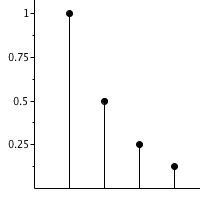
\includegraphics[scale=0.7]{img/impresp}}

  \end{floatrow}

\end{figure}

The operation that was just performed on the $\delta$ function is called "convolution". Convolution has its own mathematical symbol: $\ast$. To convolve a signal means to apply an impulse response to every of its samples. Table \ref{code:convolve} shows a C++ program to perform convolution (based on pseudo-code, see Mitchell, 2008, p. 107).\\

\begin{table}
  \code{convolve.cpp}
  \caption{A C++ function to convolve a signal vector with an impulse response vector. It should be noted that to convolve a signal vector of size $m$ with an impulse response vector of size $n$, the output vector must have a minimum size of $m + (n - 1)$.}
  \label{code:convolve}
\end{table}

\noindent The filters described so far are called Finite Impulse Response (FIR) filters, because their impulse response is of finite size, like the one shown in Figure \ref{fig:impresp}, caused by the Filter depicted in Figure \ref{fig:threedelay}. Given that in this three-sample delay filter all filter coefficients have the same value of $0.5$, the diagram could actually be re-arranged and simplified if the three delays are replaced by a single \emph{recursive} delay. Instead of processing an input sample, a recursive delay is fed an output sample, which it then amplifies or attenuates and feeds back into the signal. This re-arranged filter, also called a \emph{feedback loop}, is shown in Figure \ref{fig:iirdelay}. Because this feedback loop could theoretically go on forever, such a filter is called an Infinite Impulse Response (IIR) filter. Equation \ref{eq:iirdelay} gives a mathematical definition for the filter shown in Figure \ref{fig:iirdelay}. To prove that this filter results in the same response as the FIR filter from before, it can be fed a $\delta$ function. Because $y_{n-1}$ is initially 0, the first output $y_{n}$ will simply be $1 + \frac{0}{2}$. For the second sample, $y_{n-1}$ takes on the value of the previous output, which was 1. Therefore, the second output sample is $0 + \frac{1}{2} = 0.5$, the next sample $0 + \frac{0.5}{2}$ and so on. Because this is an IIR filter, this process could theoretically go on ad infinitum. $x_{n}$ is equal to 0 for all samples other than the first because of the way the $\delta$ function is defined.

\begin{equation}
  y_{n} = x_{n} + \frac{y_{n-1}}{2}
  \label{eq:iirdelay}
\end{equation}

\begin{figure}
  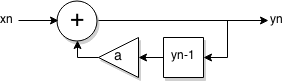
\includegraphics[scale=0.7]{img/iirdelay}
  \caption{An IIR delay filter.}
  \label{fig:iirdelay}
\end{figure}

\pagebreak

\section{Bi-Quad Filters}

A common arrangement of FIR and IIR filters is a so-called bi-quad filter. A "bi-quad filter combines one and two sample feedforward delays (FIR) with one and two sample feedback delays (IIR)". \citebs{109} Figure \ref{fig:biquad} shows such a bi-quad filter. The Equation to calculate the sample output of a bi-quad filter is given by Equation \ref{eq:biquad}.

\begin{figure}[h!]
  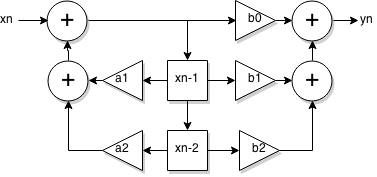
\includegraphics[scale=0.7]{img/biquad}
  \caption{A bi-quad filter.}
  \label{fig:biquad}
\end{figure}

\begin{equation}
  y_{n} = b_{0}(x_{n} - a_{1}y_{n-1} - a_{2}y_{n-2}) + b_{1}x_{n-1} + b_{2}x_{n-2}
  \label{eq:biquad}
\end{equation}

\subsection{Implementation}

In the synthesizer created for this thesis, the \texttt{Filter} class implements a bi-quad filter. Table \ref{code:filter} shows the \texttt{Filter} class' \texttt{process} method, which takes an input sample and returns a filtered output sample.

\begin{table}[h!]
  \code{filter.cpp}
  \caption{C++ function to filter an input sample and return an output sample. This function implements the bi-quad filter equation given by Equation \ref{eq:biquad}.}
  \label{code:filter}
\end{table}

\pagebreak

\section{Filter Types}

Bi-quad filters can be used to create a variety of different filter types and corresponding frequency responses, simply by adjusting the filter's coefficients. When examining a frequency response, the term \textbf{passband} is used for the frequency range that should ideally not be affected by the filter. Conversely, the \textbf{stopband} are those frequency components the filter should, ideally, silence completely. The frequency at which the transition from minimum to maximum attenuation occurs is called the \textbf{cutoff frequency} and is denoted by $f_{c}$. Because no filter is perfect, this transition usually does not happen precisely at the specified cutoff frequency. Rather, there is a certain \textbf{transition band}, which is the range of frequencies where the transition takes place. Within this transition band, the cutoff frequency is defined as the frequency component where the amplitude reaches $\frac{\sqrt{2}}{2}$ (0.707...) or -3dB in power\footnotemark. If the transition band is narrow, the filter is said to have a fast \textbf{roll-off}. If it is rather wide, the roll-off is said to be slow. Figure \ref{fig:filterterm} depicts a typical frequency response and labels the relevant bands and frequencies. It should be noted that bi-quad filters and IIR filters in general show quite slow roll-off. \citedsp{268}

\footnotetext{A signal's power is measured in decibels (dB), which is a logarithmic unit of measurement. 20dB equals an increase in amplitude by one order of magnitude ($\cdot 10$) and -20dB a decrease by one order of magnitude ($\cdot 0.1$).}

\begin{figure}[h!]
  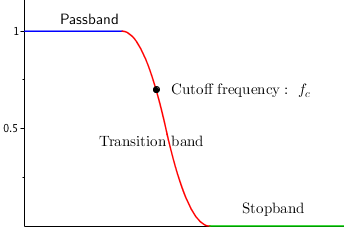
\includegraphics[scale=0.7]{img/filterterm}
  \caption{The frequency response of a filter with a relatively fast roll-off.}
  \label{fig:filterterm}
\end{figure}

\pagebreak

\subsection{Low-Pass Filters}

Low-Pass filters have their passband in the lower frequency ranges and their stopband in the higher ranges. A visualization of a low-pass bi-quad filter's frequency response when applied to a white noise signal\footnotemark{} is given in Figure \ref{fig:filterterm}.

\begin{figure}[p!]
  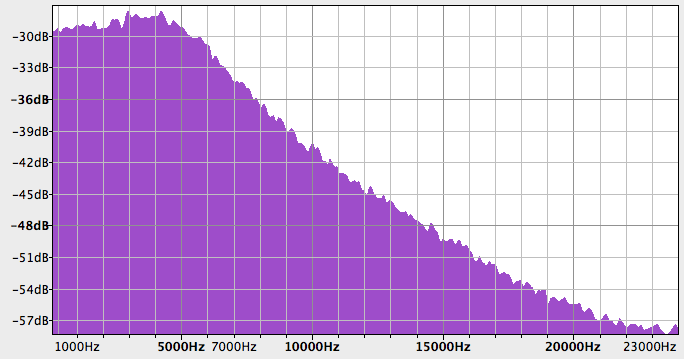
\includegraphics[scale=0.6]{img/lowpass}
  \caption{The frequency response of a low-pass bi-quad filter where $f_{c} = 5000$ Hz.}
  \label{fig:lowpass}
\end{figure}

\footnotetext{A white noise signal is used here because it has a flat frequency spectrum when un-filtered.}

\subsection{High-Pass Filters}

A high-pass filter is a low-pass filter whose spectrum has either been \emph{inverted} (flipped top-for-bottom) or \emph{reversed} (flipped left-for-right) \citedsp{271}. As a consequence, high-pass filters let high frequencies pass, while stopping lower frequencies. Figure \ref{fig:highpass} shows an appropriate frequency response.

\begin{figure}[p!]
  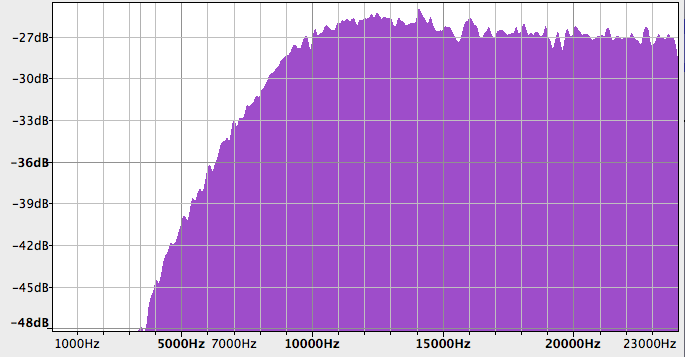
\includegraphics[scale=0.6]{img/highpass}
  \caption{The frequency response of a high-pass bi-quad filter where $f_{c} = 10000$ Hz.}
  \label{fig:highpass}
\end{figure}

\subsection{Band-Pass Filters}

Band-pass filters let frequency components in a specific range, e.g. 3000 to 5000 Hz, pass, while stopping all other frequencies lower or higher than the range of the passband. Such a filter can be created by first sending a signal through a low-pass and then through a high-pass filter. The passband of the filter created will then be the range of frequencies where the passband of the high-pass filter intersects that of the low-pass filter, since all other frequencies are in a stopband. Figure \ref{fig:bandpass} shows the frequency response of a band-pass filter.

\begin{figure}[p!]
  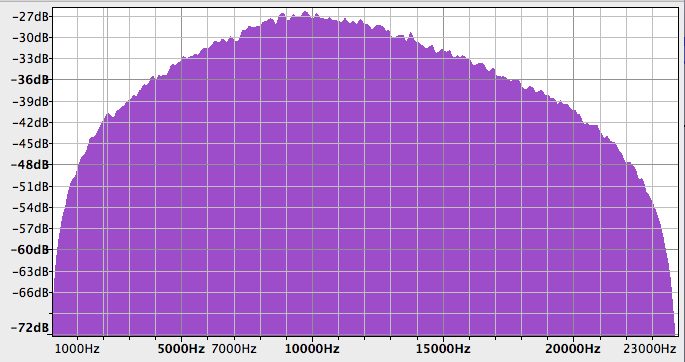
\includegraphics[scale=0.6]{img/bandpass}
  \caption{The frequency response of a band-pass bi-quad filter where $f_{c} = 10000$ Hz.}
  \label{fig:bandpass}
\end{figure}

\subsection{Band-Reject Filters}

A band-reject filter, often referred to as a "notch" filter, can be seen as the opposite of a band-pass filter. While a band-pass filter stops all frequencies except for those immediately around the cutoff frequency, a band-reject filter stops only the frequencies at the cutoff frequency and lets all others pass. Besides using the correct filter coefficients for a bi-quad filter, a band-reject filter can also be created by using a low-pass and a high-pass filter \emph{in parallel}. This involves copying a signal, then sending one copy of the original signal through a low-pass filter and the other copy through a high-pass filter. The final signal is the sum of the signal output by the high-pass filter and the signal output by the low-pass filter. Figure \ref{fig:bandreject} displays the frequency response of a band-reject filter.

\begin{figure}[p!]
  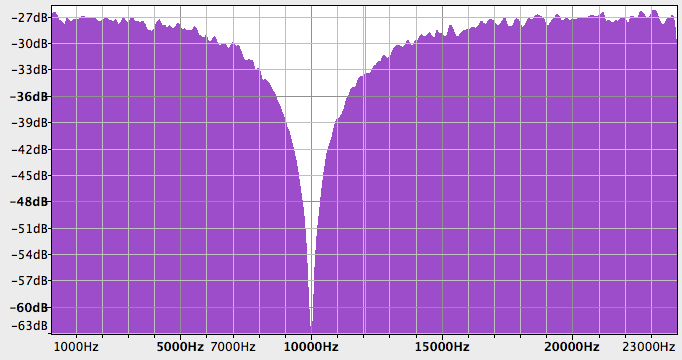
\includegraphics[scale=0.6]{img/bandreject}
  \caption{The frequency response of a band-reject bi-quad filter where $f_{c} = 10000$ Hz.}
  \label{fig:bandreject}
\end{figure}

\pagebreak

\subsection{All-Pass Filters}

A very special type of filter is the so-called all-pass filter. As its name implies, an all-pass filter lets all frequencies pass and stops none. What could possibly be the use of such a filter? The answer lies in the second alteration a filter performs on a signal: a change in phase. All-pass filters are used to change a signal's phase while leaving its amplitude un-altered at all frequencies.

\section{Filter Coefficients}

Let $\omega = \frac{2\pi f_{c}}{f_{s}}$ and $\alpha = \frac{\sin(\omega)}{2Q}$, where Q is the filter's \emph{Quality Factor}\footnotemark{}, then Table \ref{tb:coef} gives the values the various filter coefficients of a bi-quad filter must take on to achieve the wanted frequency response. These values were determined by Robert Bristow-Johnson from analog filter circuits. (Bristow-Johnson, \url{http://www.musicdsp.org/files/Audio-EQ-Cookbook.txt}, accessed 4 January 2015)

\footnotetext{The Quality Factor can be said to control to some extent the bandwith of a filter's transition band as well as the amplitude peak of the passband before transitioning to the stopband.}

\begin{table}[h!]

  \centering

  \renewcommand{\arraystretch}{3}
  \begin{tabular}[]{ | c | c | c | c | c | c |}
    \hline
    \rowcolor[gray]{0.8}
    Filter Type & $a_{1}$ & $a_{2}$ & $b_{0}$ & $b_{1}$ & $b_{2}$ \\
    \hline
    Low-Pass & $\frac{-2\cos(\omega)}{1 + \alpha}$ & $\frac{1 - \alpha}{1 + \alpha}$ & $\frac{1-\cos(\omega)}{2(1 + \alpha)}$ & $\frac{1-\cos(\omega)}{1 + \alpha}$ & $\frac{1-\cos(\omega)}{2(1 + \alpha)}$\\
    \hline
    High-Pass & $\frac{-2\cos(\omega)}{1 + \alpha}$ & $\frac{1 - \alpha}{1 + \alpha}$ & $\frac{1+\cos(\omega)}{2(1 + \alpha)}$ & $\frac{-(1+\cos(\omega))}{1 + \alpha}$ & $\frac{1+\cos(\omega)}{2(1 + \alpha)}$\\
    \hline
    Band-Pass & $\frac{-2\cos(\omega)}{1 + \alpha}$ & $\frac{1 - \alpha}{1 + \alpha}$ & $\frac{\sin(\omega)}{2(1 + \alpha)}$ & $0$ & $\frac{-\sin(\omega)}{2(1 + \alpha)}$\\
    \hline
    Band-Reject & $\frac{-2\cos(\omega)}{1 + \alpha}$ & $\frac{1 - \alpha}{1 + \alpha}$ & $\frac{1}{1 + \alpha}$ & $\frac{-2\cos(\omega)}{1 + \alpha}$ & $\frac{1}{1 + \alpha}$\\
    \hline
    All-Pass & $\frac{-2\cos(\omega)}{1 + \alpha}$ & $\frac{1 - \alpha}{1 + \alpha}$ & $\frac{1 - \alpha}{1 + \alpha}$ & $\frac{-2\cos(\omega)}{1 + \alpha}$ & $1$\\
    \hline
  \end{tabular}

  \caption{Filter coefficients for a bi-quad filter.}

  \label{tb:coef}

\end{table}
